\section{Explorative Analysis}
\begin{figure}[H]
    \vspace*{-0.7cm}
    \centering
    \subfloat[][Cats]{%
        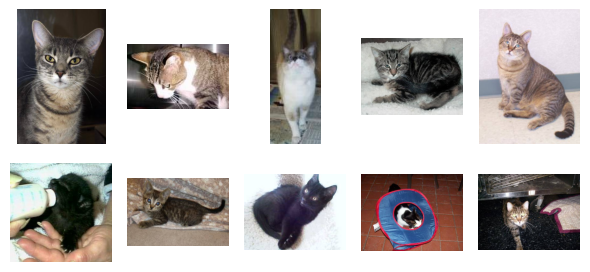
\includegraphics[width=0.35\textwidth]{figures/cats.png}\label{fig:cats}}\hspace{1cm}
    \subfloat[][Dogs]{%
        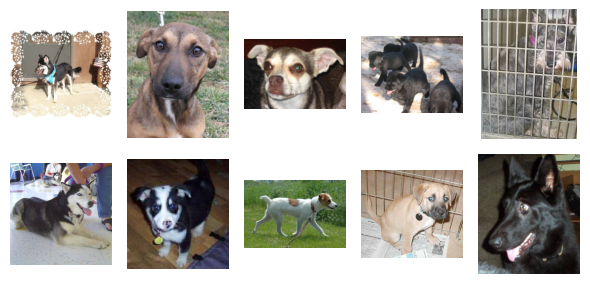
\includegraphics[width=0.35\textwidth]{figures/dogs.png}\label{fig:dogs}}
    \caption{Illustration of the effect of adaptive grids.}
    \label{fig:cats_dogs}
    \vspace*{-0.7cm}
\end{figure}

Dataset contains many diverse images and differ in terms of color, size, and orientation. The images are of varying quality, with some being clear and well-lit, while others are blurry or poorly framed. The dataset contains a mix of close-up shots and full-body shots of both cats and dogs. The dataset contains a mix of different breeds of cats and dogs, with varying fur lengths, colors, and patterns. Most of the pictures are 220-500 pixels wide, and 220-500 pixels tall. They are all in color, so they have 3 color channels. 

Cats vs. Dogs features
- Face:
- Cats generally have shorter, more rounded faces, often with triangular ears and pointed noses.
- Dogs generally have longer snouts and a greater diversity in ear shapes.
- Ears:
- Cats ears are typically upright and pointed.
- Dogs ears vary widely in shape and position, from erect to floppy, and they often have a different positioning on the head compared to cats.
- Eyes:
- Cats have generally more sharper-shaped eyes.
- Dogs have rounder eyes.
- Tail:
- Cats have long, flexible tails, often held upright or curled.
- Dogs’ tails vary greatly in length and shape, often held in different positions.
- Body Structure:
- Cats are generally lean, with flexible, agile bodies.
- Dogs come in a range of body types, from muscular to slender.
- Fur and Markings:
- Cats fur are often softer, finer, and smoother.
- Dogs often are coarser.